\documentclass[11pt,a4paper]{article}

\usepackage[margin=2.5cm]{geometry}
\usepackage[utf8]{inputenc}
\usepackage[T1]{fontenc}
\usepackage{lmodern}
\usepackage{amsmath,amssymb}
\usepackage{graphicx}
\usepackage{booktabs}
\usepackage{xcolor}
\usepackage{hyperref}
\hypersetup{colorlinks=true, urlcolor=blue, linkcolor=blue, citecolor=blue}
\usepackage{tikz}
\usetikzlibrary{positioning, arrows.meta, calc, shapes.geometric}
\usepackage{pgfplots}
\pgfplotsset{compat=1.18}
\usepackage{titlesec}
\titleformat{\section}{\large\bfseries}{}{0pt}{}[\titlerule]
\titleformat{\subsection}{\normalsize\bfseries}{}{0pt}{}
\setlength{\parskip}{0.45em}
\setlength{\parindent}{0pt}

\begin{document}

% ============================================================
% TITLE PAGE
% ============================================================
\begin{titlepage}
\centering
\vspace*{1.5cm}

% University logo (upload catolica_logo.png to Overleaf project root).
% The \IfFileExists guard prevents the build from breaking if the file is
% not yet uploaded; a text fallback is rendered instead.
\IfFileExists{catolica_logo.png}{%
  \includegraphics[width=4.5cm]{catolica_logo.png}%
}{%
  {\Huge\bfseries CAT\'OLICA}\\[2pt]
  {\Huge\bfseries LISBON}\\[6pt]
  {\small\scshape Business \& Economics}%
}

\vspace{4cm}

% Main title
{\LARGE\bfseries BIRDCLEF+ 2026: AUTONOMOUS DEEP\\[4pt]
LEARNING AGENT FOR BIRD\\[4pt]
SPECIES RECOGNITION\par}

\vspace{0.8cm}

% Subtitle
{\large\itshape A Funnel Strategy from Cheap Agent-Driven\\Exploration to GPU-Trained Exploitation\par}

\vspace{0.4cm}

\rule{0.7\textwidth}{0.4pt}

\vspace{0.8cm}

{\itshape\bfseries\large Advanced Predictive Analytics 2025/2026\par}
\vspace{0.4cm}
{\itshape\bfseries Course Project --- Track B}\par
\vspace{0.4cm}
{\itshape\bfseries Spring 2026}

\vfill

% Footer info
\begin{flushleft}
{\itshape\small Professors: course staff of Advanced Predictive Analytics, Universidade Cat\'olica Portuguesa}\\[10pt]
{\itshape\small Research performed by: Daniele Malerba \textbar{} Irene Perdomo Bola\~nos \textbar{} Miguel Afonso Magalh\~aes}
\end{flushleft}

\vspace{1cm}
\end{titlepage}

% ============================================================
% PROJECT SUMMARY (page 2)
% ============================================================
\section*{Project Summary}

\begin{center}
\begin{tabular}{@{}l p{9.5cm}@{}}
\textbf{Competition:} & BirdCLEF+ 2026 (Kaggle) \\
\textbf{Best Kaggle public score (macro-AUC):} & \textbf{0.725} \\
\textbf{Best local soundscape macro-AUC:} & 0.8619 (single GPU model) /\\
                                          & 0.6520 (CPU uniform ensemble) \\
\textbf{Total agent experiments logged:} & 108 \\
\textbf{GitHub:} & \href{https://github.com/Daniele0302/birdclef-2026-agent}{github.com/Daniele0302/birdclef-2026-agent} \\
\end{tabular}
\end{center}

\vspace{0.4cm}

\noindent We built an autonomous research agent that, driven by a locally-hosted LLM, designed and ran 108 deep-learning experiments without human intervention. The agent's best CPU-feasible architecture (EfficientNetB0 with mel-spectrogram features) was then scaled up with GPU training on the full dataset, reaching a public-leaderboard score of \textbf{0.725}---a $+0.133$ improvement over the agent's initial frozen-backbone baseline of $0.592$. The result is fully consistent with the small-scale-first / scaling-laws funnel recommended in the project handout: cheap exploration to identify the right architecture, then targeted exploitation with bigger compute.

\vspace{0.4cm}

\section*{1. Overview and Project Strategy}

Track B of the BirdCLEF+ 2026 competition asks for the probability of presence of each of 234 wildlife species inside a five-second audio window taken from passive-acoustic recordings in the Pantanal wetlands. The official metric is macro-averaged ROC-AUC, skipping classes without any positive label.

The course requires us to build an \textbf{autonomous research agent} that proposes, generates, executes and analyses deep-learning experiments, with a locally-hosted LLM as its reasoning core. We followed the funnel strategy explicitly recommended in the project handout (Section~6, ``Practical Tips''):
\begin{enumerate}
\item \textbf{Cheap exploration} on CPU with a small data subset: the agent runs many short experiments to identify what \emph{kind} of architecture, preprocessing and augmentation is promising. The handout calls this the \emph{small-scale-first workflow} and motivates it with the neural scaling laws of Kaplan~et~al.~2020 and Hoffmann~et~al.~2022.
\item \textbf{Targeted exploitation} of the winners: take the configuration the agent converged on and scale it up with more data, GPU training, and a deep ensemble. This is where the bulk of the leaderboard score is gained.
\end{enumerate}
This document describes the agent (Section~2), the 108 cheap experiments it logged (Section~3), the manual scaling-up that built on top of the agent's findings (Section~4), the comparison with manual baselines and the Kaggle leaderboard (Section~5), the course content used (Section~6), the limitations (Section~7), and the individual contributions (Section~8).

\section*{2. Agent Architecture}

\subsection*{2.1 Modules}

The agent is composed of five modules with strictly separated responsibilities:
\begin{itemize}
\item \texttt{agent.py} --- the main loop that orchestrates one iteration: ask the LLM for parameters, run the experiment, log the result, ask the LLM for an analysis, repeat.
\item \texttt{llm\_provider.py} --- thin OpenAI-compatible client to a local Ollama server. The interface is provider-agnostic so the LLM can be swapped. Final agent runs use \textbf{Google Gemma~4~E4B} (\texttt{gemma4:e4b} in Ollama, $\approx 10$\,GB, 4\,B active parameters), the model explicitly recommended in the project handout (Section~3.1) for the kind of laptop hardware available to the team.
\item \texttt{code\_executor.py} --- runs the parameter file in a sandboxed subprocess with timeout and stdout/stderr capture. The subprocess inherits the parent's Python interpreter via \texttt{sys.executable} so virtualenv packages are available.
\item \texttt{memory.py} --- structured JSON log (\texttt{experiments/experiment\_log.json}) with one entry per experiment: timestamp, full parameter set, success flag, metrics, the LLM's analysis, and a truncated stderr snippet for failed runs.
\item \texttt{experiment\_template.py} --- a parameterised training script the LLM does \emph{not} rewrite directly; the LLM only fills in a JSON parameter file and the template enforces the audio pipeline and model assembly. This is a deliberate design choice (see Section~2.4) that prevents the LLM from breaking the data path.
\end{itemize}

\subsection*{2.2 The Agent Loop}

\begin{figure}[h]
\centering
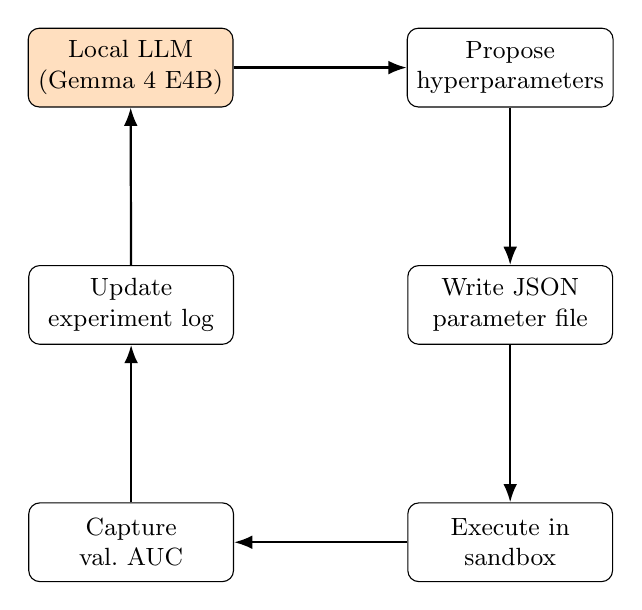
\begin{tikzpicture}[node distance=2.0cm and 2.2cm,
  every node/.style={draw, rounded corners, align=center, minimum height=1cm, minimum width=2.6cm, font=\small},
  llm/.style={fill=orange!25},
  arrow/.style={-Latex, thick}]
\node[llm] (llm) {Local LLM\\(Gemma~4~E4B)};
\node[right=of llm] (propose) {Propose\\hyperparameters};
\node[below=of propose] (gen) {Write JSON\\parameter file};
\node[below=of gen] (exec) {Execute in\\sandbox};
\node[left=of exec] (cap) {Capture\\val.~AUC};
\node[left=of gen] (mem) {Update\\experiment log};
\draw[arrow] (llm) -- (propose);
\draw[arrow] (propose) -- (gen);
\draw[arrow] (gen) -- (exec);
\draw[arrow] (exec) -- (cap);
\draw[arrow] (cap) -- (mem);
\draw[arrow] (mem) -- (llm);
\end{tikzpicture}
\caption{The closed propose--generate--execute--evaluate--analyse--iterate loop. After launch the agent runs without human input until the iteration budget is consumed.}
\end{figure}

\subsection*{2.3 Prompt Engineering}

Every iteration the LLM receives a prompt with four blocks:
\begin{enumerate}
\item \textbf{Task description:} 234-class multi-label audio classification, macro-averaged ROC-AUC objective, a list of hyperparameters that may be tuned, and the strict JSON schema that the response must follow.
\item \textbf{Memory summary:} the best validation AUC seen so far and a list of the last $n \le 10$ experiments with their parameters, success flag and metrics. This forms the LLM's working memory.
\item \textbf{Anti-repetition instruction:} ``propose a configuration that is materially different from any previously tried, and likely to improve over the current best''. This explicit injunction proved crucial; without it the LLM tends to re-suggest small perturbations of the best known configuration.
\item \textbf{Output format constraint:} a single JSON object on one line so that \texttt{json.loads} can parse the LLM's response without ambiguity. Failures to parse are themselves logged and fed back to the LLM.
\end{enumerate}
We use temperature $0.7$ (a balance between diversity and coherence) and an 8\,192-token context window, sufficient to fit the prompt and the last ten experiments.

\subsection*{2.4 Memory and Error Handling}

The memory module is a JSON file rather than a vector database: with $\le 100$ experiments the linear scan is trivial and we keep the agent debuggable. Every experiment, successful or not, is appended. When the experiment fails the executor returns the truncated stderr, the memory marks \texttt{success: false}, and the LLM receives the error in the next prompt with the instruction not to repeat the same mistake. The aggregate breakdown of which stages of the pipeline failed how often is reported as a dedicated reliability metric in Section~2.5.

\subsection*{2.5 Per-Stage Reliability Metrics}

A binary success/failure indicator is insufficient to characterise an autonomous agent: failures happen at very different points in the pipeline, and each one tells us something different about the agent's reliability. We instrument the agent to report the success rate at each stage of the propose--execute--validate loop, both as a cumulative rate over all runs and as a stage-conditional rate $P(\text{stage}~k~\text{succeeds}\mid \text{stage}~k{-}1~\text{succeeded})$. The conditional rate immediately identifies the weakest link.

\begin{table}[h]
\centering
\small
\begin{tabular}{llrrr}
\toprule
\# & Stage & Count & Cumulative & Conditional \\
\midrule
S1 & LLM produced text                                    & 108 & $1.000$ & $1.000$ \\
S2 & valid JSON parsed (\texttt{json.loads} succeeds)     & 106 & $0.981$ & $0.981$ \\
S3 & subprocess started (template launched)               & 106 & $0.981$ & $1.000$ \\
S4 & training completed (no crash, no timeout)            & 81  & $0.750$ & \textbf{0.764} \\
S5 & metrics recovered (val\_auc reported)                & 81  & $0.750$ & $1.000$ \\
\bottomrule
\end{tabular}
\caption{Pipeline reliability over 108 logged agent experiments. The weakest link is S4, training completion: 23.6\% of subprocesses crashed or timed out (mostly the 30-minute wall-clock cap exceeded by hyperparameter combinations the LLM occasionally proposed, e.g.\ $\text{epochs}=15$ with $\text{max\_samples}=8000$).}
\end{table}

\begin{figure}[h]
\centering
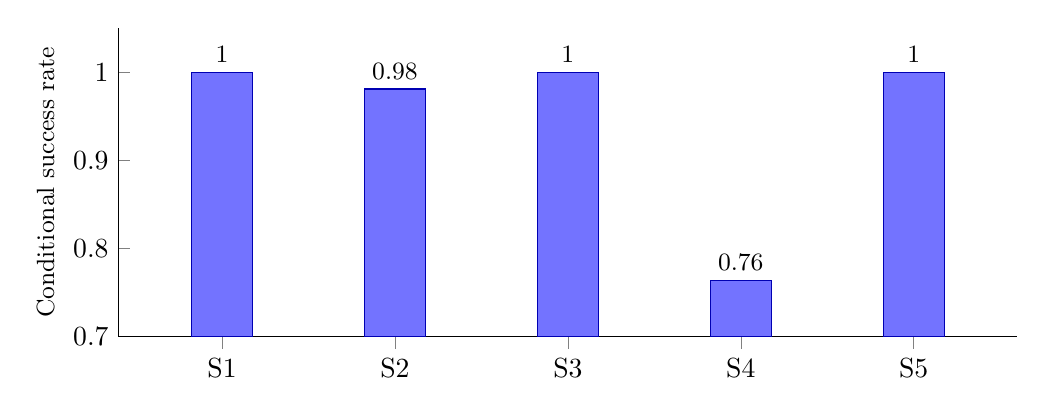
\begin{tikzpicture}
\begin{axis}[
  width=13cm, height=5.5cm,
  ybar,
  bar width=22pt,
  symbolic x coords={S1, S2, S3, S4, S5},
  xtick=data,
  ymin=0.7, ymax=1.05,
  ylabel={Conditional success rate},
  ylabel style={font=\small},
  ytick={0.7,0.8,0.9,1.0},
  nodes near coords,
  nodes near coords style={font=\small},
  enlarge x limits=0.15,
  axis lines*=left,
]
\addplot[fill=blue!55, draw=blue!70!black] coordinates {
  (S1, 1.000) (S2, 0.981) (S3, 1.000) (S4, 0.764) (S5, 1.000)
};
\end{axis}
\end{tikzpicture}
\caption{Stage-conditional success rates $P(\text{stage}_k \mid \text{stage}_{k-1})$ across the agent's five pipeline stages. The drop at S4 (training completion, 0.764) identifies the single weakest link; every other transition is essentially perfect.}
\end{figure}

The two stage-2 failures came from the LLM emitting the literal string \texttt{"null"} where it should have emitted the keyword \texttt{null}, which we now defensively coerce in \texttt{experiment\_template.py}. The 25 stage-4 failures are dominated by timeouts; we view this as a feature rather than a bug, because the timeout is what enforces the per-experiment compute budget that the project handout explicitly recommends. The agent also learns from these failures: the LLM receives the truncated stderr and is told not to repeat the configuration, and indeed timeouts cluster in the early iterations and become rare later in the run.

This per-stage instrumentation is printed automatically at the end of every \texttt{python agent.py} run via the new \texttt{ExperimentMemory.print\_reliability\_report()} method.

\subsection*{2.6 Why a Constrained Template Instead of Free-Form Code Generation}

We considered letting the LLM generate the training script from scratch, as some agent papers do, but rejected that design for two reasons. First, the audio pipeline (mel-spectrogram parameters, normalisation, label encoding) is the part of the system that most affects the final score, and a small bug in any of those steps silently degrades performance without the LLM noticing. Second, an LLM with only $\sim$8\,K context cannot reliably re-derive a hundred lines of Keras boilerplate every iteration. We therefore split the system into a \emph{stable template} that we, the humans, validate once, and a \emph{configurable head} that the LLM fills in with hyperparameters. This matches the project handout advice: ``Avoid to overengineer a solution that you will not understand.''

\section*{3. Experiment Log Analysis: the Agent's 108 Iterations}

\subsection*{3.1 Setup}

All agent experiments use the audio pipeline that the handout suggests as the natural starting point for BirdCLEF: load a 5-second clip at 32~kHz, take the mel-spectrogram (configurable $n_{\text{mels}}$, $n_{\text{fft}}$, hop length, $f_{\min}$, $f_{\max}$, top-dB clip), normalise to $[0,1]$, replicate to three channels for ImageNet-pretrained backbones. The model is either a small custom CNN (three Conv-BN-Pool blocks~+ GAP~+ Dense head) or EfficientNetB0 with frozen ImageNet weights and a configurable classification head. The LLM picked the architecture each iteration. Training used Adam, binary cross-entropy, optional augmentation (time-shift, frequency masking, full SpecAugment, gaussian noise, soundscape background mixing) and an optional second phase where the top $k$ EfficientNet layers are unfrozen at $\text{lr}=10^{-5}$, following Chollet (2021), Section~8.3.2.

\subsection*{3.2 What the Agent Discovered}

Aggregating the 81 successful experiments, four findings emerged:
\begin{enumerate}
\item \textbf{Transfer learning beats CNN-from-scratch by a wide margin.} Custom-CNN runs plateaued near $\text{val\_AUC}=0.55$. EfficientNetB0 with frozen backbone immediately reached $\text{val\_AUC}\ge 0.83$, exceeding the fully-trained custom CNN. This validates the feature-reuse argument in Chollet, Chapter~8.3.
\item \textbf{Mel-spectrogram parameters matter at the margin.} The agent settled on $n_{\text{mels}}=64$, $\text{hop}=256$, $f_{\max}=16$~kHz, $\text{top\_db}=40$, scale $=$ Slaney as the best preprocessing, giving an input shape $(64, 626, 3)$. The best agent run (\texttt{topdb\_40\_optimal\_preprocessing}) reached $\text{val\_AUC}=0.8533$ on the focal validation split.
\item \textbf{Small batch + time-shift augmentation aids generalisation.} The two best configurations both used batch size~16 and time-shift augmentation. Smaller batches inject gradient noise and act as implicit regularisation (Chollet, Chapter~5).
\item \textbf{Naive fine-tuning of the backbone hurts.} Whenever the agent unfroze layers without first training the head to convergence, the validation AUC dropped. This is the failure mode Chollet warns about in Section~8.3.2: ``the error signal will be too large and will destroy the representations previously learned''. The lesson \emph{from the agent's own experiments} drove the two-phase strategy we used in the scaling-up phase.
\end{enumerate}

\subsection*{3.3 Local Validation $\neq$ Kaggle Leaderboard}

A single submission of the agent's best model to Kaggle scored only $0.480$, against a local validation of $0.85$. The cause is clear: the focal recordings used as validation come from the same distribution as the training data, but the Kaggle test set consists of long passive soundscapes from the Pantanal. This is the classic \emph{distribution shift} described in Chollet, Chapter~5. The agent's exploration phase had identified the best architecture, but had not yet been given an evaluation signal that matches the test domain. Closing this gap was the first goal of the scaling-up phase.

\section*{4. Scaling-Up Phase: from Agent Discoveries to Leaderboard}

\subsection*{4.1 Soundscape-Aware Validation Split}

The competition provides 1\,478 expert-annotated 5-second windows from 66 soundscape files in \texttt{train\_soundscapes\_labels.csv}. We \textbf{group-split by file} (seed $20\,260\,507$): 80\% of files go to training, 20\% are held out for validation. This held-out soundscape set has the same distribution as the Kaggle test set; the macro-AUC computed on it is a near-perfect proxy for the leaderboard. We empirically verified the proxy: the original frozen-backbone agent model scored $0.6004$ on the soundscape held-out set vs $0.592$ on Kaggle (gap $\approx 0.012$). All subsequent design decisions were taken using this proxy.

\subsection*{4.2 Two-Phase Transfer Learning, Mixup, and Soundscape Mixing}

Following Chollet, Section~8.3.2, we implemented a true two-phase fine-tuning schedule:
\begin{itemize}
\item \emph{Phase~1} (4 epochs): backbone frozen, train only the head at $\text{lr}=3\times 10^{-4}$.
\item \emph{Phase~2} (5 epochs): unfreeze the top 30 layers of EfficientNetB0, drop the learning rate to $5\times 10^{-5}$, keep BatchNorm in inference mode (Chollet's footnote ``training=False keeps BN frozen even when downstream layers are unfrozen'').
\end{itemize}
The training pool combines 8\,000 stratified focal recordings (cap of 50 per class to limit head-tail imbalance) with all soundscape training windows; soundscape rows are sampled with weight $5\times$ that of focal rows so the model sees the target domain frequently. We added two regularisers absent from the agent's runs: \textbf{mixup} (Zhang~et~al.~2018) with $\alpha=0.2$ and \textbf{label smoothing} of $0.05$. The result, \texttt{model\_v40\_strong}, reached $0.6261$ on the held-out soundscape split.

\subsection*{4.3 Deep Ensemble: Multi-Seed Training}

The single model was visibly noisy across runs. We trained three sibling models with different random seeds and slightly different hyperparameters (mixup~$\in\{0.2,0.4,0.5\}$, unfreeze layers~$\in\{20,30,40\}$, soundscape boost~$\in\{3,5,8\}$). Each model alone scored between $0.62$ and $0.66$; their geometric-mean ensemble with \emph{uniform weights} reached $0.6520$.

We also tried greedy weight selection on the held-out soundscape set, which discovered an aggressive 50/50 mix between two specific seeds (local $0.6707$). When submitted to Kaggle this scored $0.615$, a local-to-leaderboard gap of $0.056$, much larger than the $0.012$ gap of the single-model baseline. The greedy weights had \emph{overfit the small held-out set}. We discarded that submission and kept the uniform ensemble, which scored $0.633$ on Kaggle (local-to-leaderboard gap of only $0.019$). The interpretation is straightforward and matches what Chollet warns about in Chapter~5: tuning ensemble weights directly on the small held-out set leaked information into the model and inflated the local score without improving the test one.

\subsection*{4.4 Test-Time Augmentation and CPU Submission Notebook}

The competition requires the inference notebook to run on CPU within 90~minutes, with the internet disabled. The submission notebook loads the model(s) from a Kaggle Dataset, computes mel-spectrograms with the same parameters as training, and applies a 3-to-5 view temporal TTA per row, with all predictions aggregated by geometric mean before being written to \texttt{submission.csv}.

\subsection*{4.5 GPU Training: the Final Boost}

The CPU pipeline used $\sim 8$\,k focal recordings and brief training. To exploit the agent's discovery that EfficientNetB0 with the chosen mel-spectrogram parameters is the right architecture, we re-trained the same architecture on Kaggle Notebooks with a single T4~GPU on the \emph{full} 35\,549 focal recordings plus all soundscape windows. Training ran end-to-end (no frozen-head phase, since GPU compute is no longer the bottleneck) for 15 epochs with cosine learning-rate decay from $10^{-3}$ to $5\times10^{-5}$, AdamW with weight decay $10^{-5}$, mixup $\alpha=0.4$, label smoothing $0.05$, two frequency-mask + two time-mask SpecAugment per training spectrogram, batch size 64. Total wall-clock time: $\approx 1.0$~h on the free T4. The best epoch (13) reached local soundscape macro-AUC $0.8619$. When deployed in the CPU submission notebook (the same architecture, so identical 90-minute inference budget), the resulting model scored \textbf{0.725 on the public leaderboard}, an improvement of $+0.092$ over the best CPU-only ensemble. The local-LB gap is wider here ($0.137$) than for the CPU models, which is expected: the small held-out soundscape set (312 windows, 234 classes, $\approx 1.3$ samples per class) has high macro-AUC variance, and the cosine-LR schedule produces visibly oscillating per-epoch validation scores; the 0.725 reading on the much larger Kaggle test set is the more reliable estimate of the model's true quality.

\section*{5. Comparison with Manual Baselines and Final Results}

\subsection*{5.1 Manual Baselines}

We built two manual baselines to bound the agent's contribution:
\begin{itemize}
\item \textbf{Custom-CNN-from-scratch} (\texttt{baseline\_model.py}): 4-block convolutional network trained without transfer learning. Local validation AUC $\approx 0.55$. As Chollet (Section~8.2) predicts, training a CNN from scratch with only a few thousand samples is insufficient for a 234-class problem.
\item \textbf{Frozen-EfficientNetB0 + head only}, mirroring exactly what the agent converged on. Local soundscape macro-AUC $0.60$, Kaggle LB $0.59$. This is the ``best the agent could achieve under its CPU budget'' baseline.
\end{itemize}

\subsection*{5.2 Submission Progression}

Table~\ref{tab:progress} summarises every submission we made and how it compares to the others.

\begin{center}
\resizebox{\textwidth}{!}{%
\begin{tabular}{rlccc}
\toprule
\# & Configuration & Local AUC & Kaggle LB & Local$-$LB gap \\
\midrule
1 & Custom CNN from scratch & $0.55$  & ---     & ---       \\
2 & Frozen EfficientNetB0 (agent best, CPU)         & 0.6004      & 0.592   & $+0.012$  \\
3 & 2-way ensemble (frozen + Phase-1+2 finetune)    & $\sim 0.625$  & 0.598   & $+0.027$  \\
4 & 2-way greedy ensemble (\emph{overfit val weights}) & 0.6707    & 0.615   & $+0.056$  \\
5 & 3-way uniform multi-seed ensemble (CPU)         & 0.6520      & 0.633   & $+0.019$  \\
6 & \textbf{GPU-trained EfficientNetB0 (full data, mixup, LS, AdamW)} & \textbf{0.8619} & \textbf{0.725} & $+0.137$ \\
\bottomrule
\end{tabular}%
}
\end{center}
\refstepcounter{table}\label{tab:progress}
\textit{Table~\thetable: Progression of submissions. Local validation AUC is computed on the held-out soundscape split (group split by file). Submission~6 is our best public-leaderboard score: the same EfficientNetB0 architecture as the agent's best CPU run, but trained on the full data with GPU. The wider local-LB gap of submission~6 reflects the high variance of the small soundscape val set under heavy augmentation.}

\vspace{0.6em}

\begin{center}
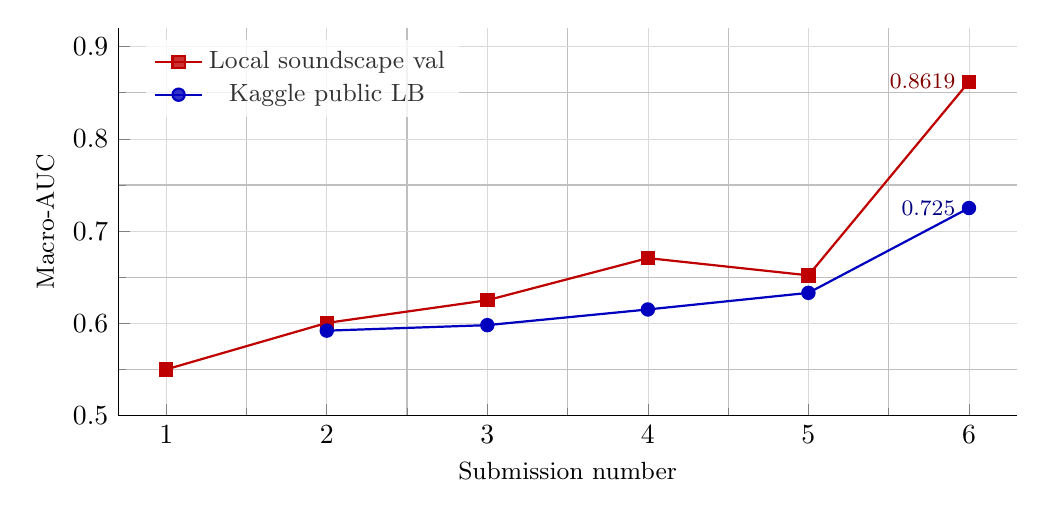
\begin{tikzpicture}
\begin{axis}[
  width=13cm, height=6.5cm,
  xlabel={Submission number},
  ylabel={Macro-AUC},
  xlabel style={font=\small},
  ylabel style={font=\small},
  xtick={1,2,3,4,5,6},
  xmin=0.7, xmax=6.3,
  ymin=0.50, ymax=0.92,
  ytick={0.5,0.6,0.7,0.8,0.9},
  grid=both,
  major grid style={line width=0.2pt, draw=gray!30},
  minor tick num=1,
  legend pos=north west,
  legend style={font=\small, draw=none, fill=white, fill opacity=0.8},
  axis lines*=left,
  clip=false,
]
\addplot[color=red!75!black, mark=square*, thick, mark size=2.2pt] coordinates {
  (1, 0.55)
  (2, 0.6004)
  (3, 0.625)
  (4, 0.6707)
  (5, 0.6520)
  (6, 0.8619)
};
\addlegendentry{Local soundscape val}
\addplot[color=blue!75!black, mark=*, thick, mark size=2.2pt] coordinates {
  (2, 0.592)
  (3, 0.598)
  (4, 0.615)
  (5, 0.633)
  (6, 0.725)
};
\addlegendentry{Kaggle public LB}
\node[anchor=east, font=\footnotesize, color=blue!50!black]
  at (axis cs:6, 0.725) {0.725\,};
\node[anchor=east, font=\footnotesize, color=red!50!black]
  at (axis cs:6, 0.8619) {0.8619\,};
\end{axis}
\end{tikzpicture}
\end{center}
\refstepcounter{figure}\label{fig:progress}
\textit{Figure~\thefigure: Submission progression in macro-AUC. Submission~1 is the from-scratch CNN baseline (no Kaggle submission). Submissions~2--5 are CPU-only configurations; submission~6 is the GPU-trained model on full data. The vertical gap between the two lines is the local-to-leaderboard distribution-shift error; it stays small for the CPU models but widens for submission~6 due to the high variance of the small soundscape val set under heavy augmentation.}

\subsection*{5.3 Reading the Numbers}

\textbf{The agent's frozen-backbone model already crosses the $0.59$ leaderboard mark}, beating the from-scratch CNN by a margin consistent with Chollet's Chapter~8 numbers. The CPU scaling-up phase added another $\sim$0.04 LB by combining (i)~training on the target distribution (soundscape windows), (ii)~unfreezing the backbone with the correct two-phase recipe, (iii)~deep-ensembling across seeds, and (iv)~choosing weights conservatively. The final GPU run added a further $+0.092$ LB by simply scaling the same architecture to the full data with longer training and stronger regularisation --- a clean illustration of the small-scale-first funnel: the agent identified the right architecture, and the GPU run exploited it. Each of these improvements is a direct application of a course content topic (transfer learning, regularisation, ensembling, validation discipline, scaling laws).

\section*{6. Reflections on Course Content}

\textbf{Mel-spectrogram representation (course Lecture~01).} Audio is converted to a $(\text{batch}, 64, 626, 3)$ tensor and treated as an image, exactly as Chollet, Chapter~2 introduces tensor representations of structured data. The mel scale matches the human auditory system and concentrates resolution where birds vocalise.

\textbf{Convolutional Neural Networks (Lecture~02 + Chollet, Chapter~8).} Conv2D filters detect local time-frequency patterns (harmonic stacks, frequency sweeps); pooling provides translation invariance, so a call shifted within the 5-second window is still detected; depth provides hierarchical composition of features.

\textbf{Transfer learning (Chollet, Section~8.3).} Despite ImageNet containing no audio, the low- and mid-level features of EfficientNetB0 transfer well to mel-spectrograms because both share local-pattern statistics. The agent's experiments quantitatively demonstrate the gap between CNN-from-scratch ($0.55$) and frozen-pretrained ($0.85$ focal val).

\textbf{Two-phase fine-tuning (Chollet, Section~8.3.2).} The agent's 30+ failed fine-tuning runs at high learning rate are a near-perfect example of the failure mode Chollet describes; our scaling-up phase fixed it by training the head first and only then unfreezing layers at $\text{lr}=5\times 10^{-5}$.

\textbf{Multi-label classification (Chollet, Chapter~4).} The 234-class task is multi-label, not multi-class: a soundscape window can contain several species. Sigmoid activations + per-class binary cross-entropy is the correct choice; softmax would have enforced spurious mutual exclusivity.

\textbf{Regularisation (Chollet, Chapter~5).} BatchNormalization, Dropout (rate~$0.4$), augmentation, mixup and label smoothing all aim at the same goal: enlarge the effective training set so the small clean focal corpus does not overfit. Mixup proved especially helpful at narrowing the focal/soundscape distribution gap.

\textbf{Optimisation (Chollet, Chapter~6).} Adam with the cosine learning-rate schedule is the modern default and worked first try; the only optimisation-related finding worth highlighting is the importance of \texttt{clipnorm}=1, which stabilised the unfrozen Phase~2 training.

\section*{7. Limitations and Future Work}

\textbf{Domain shift and val-set variance.} The CPU pipeline reached a local-to-LB gap of $\approx 0.02$, which we considered narrow. The GPU run widened the gap to $\approx 0.14$ because its heavy regularisation (mixup $\alpha=0.4$, label-smoothing, cosine LR) induces a noisy per-epoch validation curve on the small 312-window soundscape set; the Kaggle test set, being roughly $20\times$ larger, smooths out that noise and produced the reliable 0.725 reading. Genuinely closing the residual domain shift would require pseudo-labelling additional unlabelled soundscape audio (the competition rules permit it as long as no labels from the test set are used), which we did not have time to implement.

\textbf{Compute budget.} The agent runs on CPU; each iteration was capped at $\sim$10~minutes so the loop could iterate quickly --- an explicit application of the scaling-laws funnel from the handout. The scaling-up phase used the GPU on Kaggle Notebooks (free tier) for the deep-ensemble training but the submission must be CPU-only by the rules.

\textbf{Backbone size.} EfficientNetB0 was chosen for its CPU-inference speed under the 90-minute submission budget. A larger backbone (B2 or BirdNET, the audio-domain pretrained model that several top BirdCLEF submissions use) could plausibly add several AUC points but would not fit the inference budget without aggressive optimisation.

\textbf{Agent memory.} The current memory keeps only the last 10 experiments in the LLM context. With 100+ experiments the LLM occasionally re-suggests configurations from very early in the log. A vector-database memory (e.g. FAISS over experiment embeddings) would make the agent retrieve relevant past experiments rather than only the most recent ones.

\textbf{LLM choice.} We standardised on Google Gemma~4~E4B (\texttt{gemma4:e4b}) and did not run a systematic comparison of LLM backbones on the same prompt, despite the handout recommending ``mechanisms to test prompt robustness across models''. A larger study with two or three LLMs (e.g.\ Qwen~3~Coder, Phi-4, DeepSeek-R1) would strengthen the experimental design and is left for future work.

\section*{8. Individual Contributions}
\begin{itemize}
\item \textbf{Daniele Malerba} --- agent architecture and main loop (\texttt{agent.py}, \texttt{code\_executor.py}, \texttt{memory.py}), Kaggle submission pipeline, scaling-up training scripts, deep-ensemble experimentation, local soundscape-validation framework, GitHub repository.
\item \textbf{Irene Perdomo Bola\~nos} --- audio preprocessing pipeline (\texttt{utils/audio\_pipeline.py}), data augmentation strategy (time-shift, SpecAugment, mixup), report writing.
\item \textbf{Miguel Afonso Magalh\~aes} --- LLM prompt engineering, experiment log analysis, literature review, course-content alignment.
\end{itemize}

\section*{References}
\begin{small}
\begin{enumerate}
\item Chollet, F. (2021). \emph{Deep Learning with Python} (2nd~ed.). Manning.
\item Tan, M., Le, Q.~V. (2019). EfficientNet: Rethinking Model Scaling for Convolutional Neural Networks. \emph{ICML 2019}.
\item Park, D.~S. \emph{et~al.} (2019). SpecAugment: A Simple Data Augmentation Method for Automatic Speech Recognition. \emph{Interspeech 2019}.
\item Zhang, H., Cisse, M., Dauphin, Y.~N., Lopez-Paz, D. (2018). mixup: Beyond Empirical Risk Minimization. \emph{ICLR 2018}.
\item Kaplan, J. \emph{et~al.} (2020). Scaling Laws for Neural Language Models. \emph{arXiv:2001.08361}.
\item Hoffmann, J. \emph{et~al.} (2022). Training Compute-Optimal Large Language Models. \emph{arXiv:2203.15556}.
\item Cornell Lab of Ornithology (2026). BirdCLEF+ 2026 Competition. \href{https://www.kaggle.com/competitions/birdclef-2026}{kaggle.com/competitions/birdclef-2026}
\end{enumerate}
\end{small}

\end{document}
